\documentclass[a4paper, 10pt, conference]{ieeeconf}    
\IEEEoverridecommandlockouts                         \overrideIEEEmargins                                     
\usepackage{graphics} % for pdf, bitmapped graphics files
\usepackage{epsfig} % for postscript graphics files
\usepackage{mathptmx} % assumes new font selection scheme installed
\usepackage{times} % assumes new font selection scheme installed
\usepackage{amsmath} % assumes amsmath package installed
\usepackage{amssymb}  % assumes amsmath package installed
\usepackage{hyperref}

\title{\LARGE \bf
BLG 454E Learning From Data\\ Term Project Report
}


\author{150120145 Furkan Er, 150120914 Emin Mastizada, 150140138 Halit Uyanik}

\begin{document}

\maketitle
\thispagestyle{empty}
\pagestyle{empty}

%%%%%%%%%%%%%%%%%%%%%%%%%%%%%%%%%%%%%%%%%%%%%%%%%%%%%%%%%%%%%%%%%%%%%%%%%%%%%%%%
\begin{abstract}

An important part of business is to decrease the amount of unnecessary cost as much as possible. An example case of a business model analysis is done in this paper. A customer shipment data is given with features and corresponding labels. It is expected to calculate the possible outcome for provided test data after training our network.

\end{abstract}

%%%%%%%%%%%%%%%%%%%%%%%%%%%%%%%%%%%%%%%%%%%%%%%%%%%%%%%%%%%%%%%%%%%%%%%%%%%%%%%%
\section{INTRODUCTION}

An employee has recieved a task about analysing a data set, and making future predictions whether a customer will return their shipment or not. In order to accomplish this goal, employee needs to clean and train its data, then fit this data into his/her model.

Following are our Kaggle names: Halit U., Emin Mastizada, and F. Er. Our team name is
150120914\_150120145\_150140138 which consists our Student IDs. At the time this paper is written, our score is 849.0, and our rank is 2. Note that this might change for better or worse after the private data part of the ladder is announced.

\section{DATA SET USED}

Train data consists of 13 features: orderItemID, orderDate, deliveryDate, itemID, size, color, manufacturerID, price,customerID, salutation, dateOfBirth, state, creationDate, and 1 label: returnShipment. Figure 1 shows how many missing fields each one of the columns have in the data. Data takes 36.7 MB in the memory according to info from pandas DataFrame object.



\begin{table}[h]
	\centering
	\begin{tabular}{ l l l l }
		\hline
		\begin{tabular}[c]{@{}l@{}}Feature \\ Names\end{tabular} & Data Type & \begin{tabular}[c]{@{}l@{}}Data \\ Context\end{tabular} & \begin{tabular}[c]{@{}l@{}}Missing \\ Value \\ Count\end{tabular} \\ \hline
		orderItemID                                              & integer   & 1 2 3 4 5 6 7...                                        & 0                                                                 \\ \hline
		orderDate                                                & string    & "2012-04-01"...                                         & 0                                                                 \\ \hline
		deliveryDate                                             & string    & "1990-12-31"...                                         & 39419                                                             \\ \hline
		itemID                                                   & integer   & 186 71 71 ....                                          & 0                                                                 \\ \hline
		size                                                     & string    & "1", "10", "10+"....                                    & 0                                                                 \\ \hline
		color                                                    & string    & "almond","amethyst",..                                  & 143                                                               \\ \hline
		manufacturerID                                           & integer   & 25 21 21 14 53 87 1 3 ...                               & 0                                                                 \\ \hline
		price                                                    & float     & 69.9 70 70 39.9 ...                                     & 0                                                                 \\ \hline
		customerID                                               & integer   & 794 794 794 ....                                        & 0                                                                 \\ \hline
		salutation                                               & string    & "Company", "Family" ...                                 & 0                                                                 \\ \hline
		dateOfBirth                                              & string    & "1655-04-19", ....                                      & 48889                                                             \\ \hline
		state                                                    & string    & "Baden-Wuerttemberg",..                                 & 0                                                                 \\ \hline
		creationDate                                             & string    & "2011-02-16", ....                                      & 0                                                                 \\ \hline
		returnShipment                                           & integer   & "0", "1"                                                & 0                                                                 \\ \hline
	\end{tabular}
	\caption{Information for Shipment Data}
\end{table}

However some fields such as date fields are given as string and therefore, needs to be converted to a suitable object type for processing. This is handled by using datetime library of Python programming language to convert string to datetime whenever needed.

Second problem on base training set was missing values. There were three columns which had missing values on them. These columns are deliveryDate, color, and dateOfBirth, while [1] suggests that dateOfBirth column has too many values missing to be replaced with, we had to do it in order to calculate possible results for all data rows. First unique customerID indices were pulled from data, then from the available date of birth values, an average is calculated and '?' are replaced with this average value. Second thing is as [1] mentions, some values are too old to be alive, so we also replaced them with this average value.

Missing deliveryDate data is replaced with the average value of all other order and delivery dates. Missing colors are replaced with the most commonly occuring color, and date of birth is replaced with the average value of all customers.

Third problem was the strings which are hard to process without converting to a numerical data type. These columns include size, color, salutation, and state. In order to solve this problem, we have used mapping on unique strings. An example is, if we had black, red, and yellow for color types, we numbered all black, red, and yellows as 0, 1, 2. After that since all values are numerical, we can use them as our model feature inputs.

\subsection{Useful New Features}

After converting our base features to numerical types, next goal was to find possible new features from this data. 8 new features are pulled from our training set [1]. These are: 
\begin{itemize}
	\item Age of each customers account.
	\item Age of each customer
	\item Delivery time of each product
	\item Distance of the delivery to new years eve
	\item Distance of the delivery to lovers date
	\item Average price paid per user
	\item Ratio of a persons total purchase and returned count
	\item Purchased item count per user
	\item Risk of an item being returned depending on itemID
	\item Risk of an item being returned depending on customerID
	\item Risk of an item being returned depending on manufacturerID
\end{itemize}

First 5 features are self explanatory. However it might be better to give a brief information about the risk calculation. The calculation is taken from [1], main idea is to calculate the risk in a way that it is less affected from the products which also sold less than the others. This improves the reliabilty of the feature. Risk formula is:
\bigbreak
$
risk = 1 - \frac{r_0^c + 50}{(r_0 + r_1)^c + 100}
$
\bigbreak
r0 and r1 represents whether the product is returned or not.

\section{METHODS USED}

Python and its famous data analysis and visual libraries, numpy, tabulate, datetime, dateutil, pandas, and sklearn are used for processing both train and test data. Pandas dataframe allows user to easily manupilate the data however needed, and it also provides useful class utilities.
\bigbreak
We have tried several different models to train our data, it would take too much space here but, table 1 shows the comparison of several models depending on their results from Kaggle, we have not included the models which we couldnt get any outputs:
\bigbreak

\begin{table}[h]
	\centering
	\begin{tabular}{|r|r|}
		\hline
		\multicolumn{1}{|c|}{Model} & \multicolumn{1}{c|}{Kaggle Result} \\ \hline
		RandomForestClassifier      & 849                                \\ \hline
		ExtraTreeRegressor          & 1050                               \\ \hline
		Native bagging              & 3514                               \\ \hline
		Random Forest Regressor     & 3550                               \\ \hline
		MLPClassifier               & 7000                               \\ \hline
		PassiveAggressiveClassifier & 8600                               \\ \hline
		Deep Neural Network + Adam Optimizer & 8782                      \\ \hline
		SGD Classifier              & 10600                              \\ \hline
		MultinomialNB               & 11000                              \\ \hline
	\end{tabular}
	\caption{Different Models and Their Kaggle Results}
	\label{my-label}
\end{table}

As can be seen from Table 1, RandomForestClassifier gave the best result among other models. There might be some other model out there we have yet to heard of, therefore we do not claim this to be best fit for this data. Also we couldn't get better results from SVM Classification and Regression models (best accuracy was 60\%) and it took an hour for a 50\% of of the training set Using PCA to reduce components also not helped due to its complexity $O(n_{samples}^2 * n_{features})$.

We used 2D linear graphs for each features and ignored all ID columns, that helped us to pick useful columns.

\subsection{RandomForestClassifier}

Random forest classifier is an ensemble algorithm which the source code can be seen under sklearns documentation. A random forest classifier shows its power by creating different decisions from the random samples of the data, then choosing the best results among those in terms of accuracy.

Random forest classifier can have a lot of estimators(trees), but due to memory issues in our computers, we limited this value to 50. Also it should be noted that instead of using the default 'gini' criterion in sklearn, we used the 'entropy' criterion.

\begin{figure}[ht]
\centering
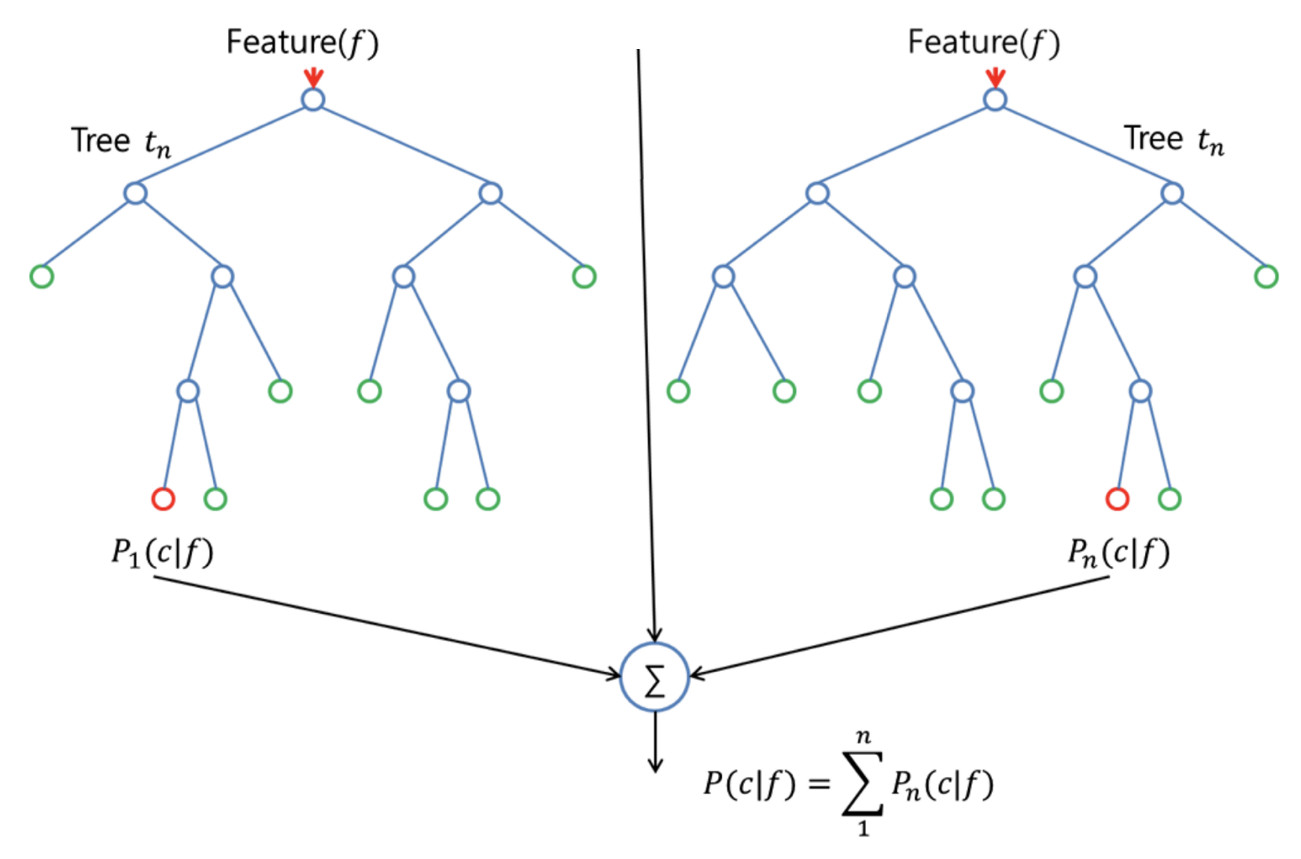
\includegraphics[width=8cm]{randomforest}
\caption{Random Forest Classifier}
\end{figure}

\subsection{Deep Neural Network}

Deep Neural Network is network of nodes (neurons) between input data and output label. Using backpropagation it calculates weights for each input node. For our example we designed 2 hidden layers, 100 neurons in first one, 50 neurons in the second layer. Accuracy results were 65%. Neuron sizes were estimated using Titanic example.

\begin{figure}[ht]
\centering
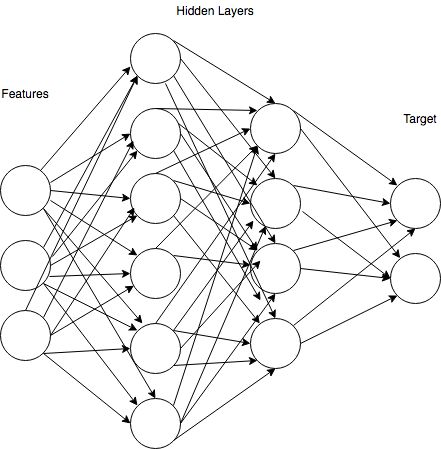
\includegraphics[width=8cm]{DNN}
\caption{Deep Neural Network}
\end{figure}

\section{RESULTS}

Since our group didnt have access to the test returnShipment data on Kaggle, we have obtained our results using the dataset given to us. We have separated the data into 2 portions, one portion for training which consists 90 percent, and another portion for testing which is 10 percent of the data. Reason for why we choose the numbers this way is because the test set given to us have 50078 rows. This is nearly 10 percent of our initial data.

Also, an important side note here is that, since we divided our initial data, sometimes a set included come unique identifiers such as a color string. This made it quite random for mapping functions to succeed, so tests are run again and again till they succeed. It might be possible to add unnecessary noise to data if we preprocessed both training and test sets together. This shouldnt be too important unless the data separation ratio is high.

Accuracy score is used to calculate the accuracy between our separated test and training data from the initial data. RandomForestClassifier gave \%70 accuracy on our local tests.

\section{CONCLUSIONS}

After cleaning our data properly, customer-order data is successfully trained and fit into our mentioned model. New features are produced in order to get a better understanding between the different relations in the models. How the random forest classifier works is explained in terms of its importance in our project. Then results and final comments are given for the experimentation.

A further improvement on this work can be done with finding new features from the original data. Doing so will improve the accuracy of further trainings, and it might be possible that some of the features we included in this work will turn out to be unnecessary.

The source code for our experiments is published in \href{https://github.com/mastizada/lfd2018/}{Github}

\bibliographystyle{ieeetr}
\bibliography{report}




\end{document}
